\section{MultiLayer Perceptron (30 pts)}

In this problem we will implement multi-layer perceptron for an image classification task. The data we use here is a subset of the CIFAR-10 dataset\footnote{\url{https://www.cs.toronto.edu/~kriz/cifar.html}}, where there are 10 classes of $32\times32$ images.

\fbox{%
    \parbox{\textwidth}{%
        \textbf{Warning: }It takes \textit{multiple hours} to train all of the  networks. Please start early and leave ample time for training/debugging. Be sure to \textit{vectorize} all of your computations to ensure they can run fast enough (so make computations in the form of vector and matrix multiplications as much as possible instead of for loops).\\\\
        In \textbf{Problem 5 and 6}, you will first implement several classes of important neural network modules, and then use these modules to build up the networks. For this part, we provide a template code. Please FOLLOW the templates, and implement the classes methods. Do NOT change the interface. The classes will be used for auto-grading. Code that does not pass the autograder WILL NOT be graded.
    }%
}

{\bf Format of the data}: 
The dataset are stored in a pickle file (\texttt{cifar10-subset.pkl}), which can be downloaded from the ``Resources'' tab on piazza. There are 5000 images for training and 2000 images for testing, each corresponding to an ``integer'' label (in range $0$ to $9$). Once you download the dataset, replace \texttt{CIFAR\_FILENAME} in the main function by the relative path you store the pickle file. \texttt{trainX} is a numpy array of dimension $(5000, 3072)$ representing the 5000 training images, and \texttt{trainy} is a $(5000, 10)$ dimensional numpy array of one-hot vectors representing the corresponding label information. Similarly, \texttt{testX} and \texttt{testy} contain $2000$ data points and use the same format as the training dataset (i.e, $(2000, 3072)$ dimensional array and $(2000, 10)$ dimensional array). Normalizing the input (\texttt{trainX}, \texttt{testX}) to [0, 1] and converting the input to numpy array of float32 can accelerate training.

The label mappings are:
\begin{verbatim}
    { 
      0: `Airplane', 
      1: `Automobile',
      2: `Bird',
      3: `Cat',
      4: `Deer',
      5: `Dog',
      6: `Frog',
      7: `Horse',
      8: `Ship',
      9: `Truck',
    }
\end{verbatim}

%The data is stored in multiple pickle files, with 10000 images for training and 2500 for testing. It can be found on Piazza under the Resources tab. Once you download the dataset, replace \texttt{SVHN\_DOWNLOAD\_PATH} of \texttt{load\_svhn.py} with the directory where you extracted the dataset. Each image's class corresponds to a specific digit (ranging from $0$ to $9$). \texttt{train\_X.npy} is a Numpy array of dimension $(10000, 3072)$ representing the 10000 training images, and \texttt{train\_y.npy} is a $(10000,)$ dimensional Numpy vector containing the corresponding labels for the images. Similarly, \texttt{test\_X.npy} and \texttt{test\_y.npy} contain $2500$  datapoints and use the same format as the training dataset (i.e, $(2500 \times 3072)$ dimensional array and $(2500,)$ dimensional vector). The pixel values of the images (\texttt{train\_X}, \texttt{test\_X}) are already normalized to [0, 1].


% \footnote{Download: \url{https://drive.google.com/drive/folders/1y1s2ddGSgClJbd3QHHqHS12lNe48q7vx?usp=share_link}}

As a warm up practice (not graded), we recommend loading the data and plotting a few examples. 

\textbf{For problems 5 and 6, submit \texttt{mlp.py} and \texttt{cnn.py} only to gradescope (select them simultaneously and drag them to upload).}



\subsection{Implementation (15 pts)}

In the Problem 5 folder, \textbf{mlp.py} is the only file you need to work on. \textbf{tests.py} and \textbf{tests.pk} are to help you test your implementation locally. Passing these local tests does not guarantee you passing the final online auto-grading tests, but failing locally very likely means also failing online. The following are terminal commands to run single module test and all modules test. 
\begin{verbatim}
    python -m unittest tests.TestReLU
    python -m unittest tests
\end{verbatim}

In \textbf{mlp.py}, there is a base class called \texttt{Transform} which you do not need to change. The \texttt{Transform} class represents a procedure done to some input $X$. In symbolic terms, $out = f(X)$, where $f$ represents the transformation, $y$ the output, $x$ the input. We will be implementing the basic layers (e.g. \texttt{ReLU}, \texttt{LinearMap}, etc.) of neural networks by inheriting this \texttt{Transform} base class.


Below is a list of classes we will implement. Implement wherever the code template says \texttt{pass}. Reading \texttt{tests.py} might help you debug your implementation. 

\begin{itemize}
    \item {\bf ReLU} ({\bf 1 point}): The layer of Rectified Linear Unit, a popular activation function. Available unit tests: \texttt{TestReLU};
    
    \item {\bf LinearMap} ({\bf 3 points}): Linear Transformation layer, i.e. fully-connected layer. In parameter update function \texttt{step()}, parameters should be updated using gradient descent with momentum. Available unit tests: \texttt{TestLinearMap};
    
    \item {\bf SoftmaxCrossEntropyLoss} ({\bf 2 points}): The layer of softmax and cross-entropy loss. The input is the pre-softmax logits, and the output is the \textbf{mean} cross-entropy loss across samples in a batch. Available unit tests: \texttt{TestLoss};
    
    \item {\bf SingleLayerMLP} ({\bf 3 points}): This is a nerual network with one hidden layer. The output is the logits(pre-softmax) for the classification tasks. Available unit tests: \texttt{TestSingleLayerMLP};
    
    \item {\bf TwoLayerMLP} ({\bf 3 points}): This is a neural network with two hidden layers. The output is the logits(pre-softmax) for the classification tasks. Available unit tests: \texttt{TestTwoLayerMLP}.
    
    \item {\bf Dropout} ({\bf 1 point}): The dropout layer. In this assignment, we apply mask and scaling during training and do nothing at test time. Available unit tests: \texttt{TestDropout}.
    
    \item {\bf BatchNorm} ({\bf 2 points}): The batch normalization layer. Please refer to the batch normalization paper or this\footnote{\url{https://agustinus.kristia.de/techblog/2016/07/04/batchnorm/}} for implementation. Available unit tests: \texttt{TestBatchNorm}.
\end{itemize}
\pagebreak
\textbf{Tips}:
\begin{itemize}
    \item LinearMap layer weights should be initialized using Xavier Initialization:
        \[W^k_{i,j}\sim\texttt{Uniform}(-b,b) \;,\quad b=\sqrt{\frac{6}{m+n}}\]
     where $k$, $i$, $j$ are indices for network layer and nodes, $m$ and $n$ are the input and output dimension;
    \item Special practices might be necessary for the numerical stability of the Softmax function;
   % \item You can start with these hyperparamters. Learning rate: 0.001, $\alpha$: 0.9 (parameter for momentum), batch size: 128. Other hyperparameters very likely could give better performance. Hyperparameters should be consistent when you compare different network architectures. 
\end{itemize}

This is what the TwoLayer network would look like:\\
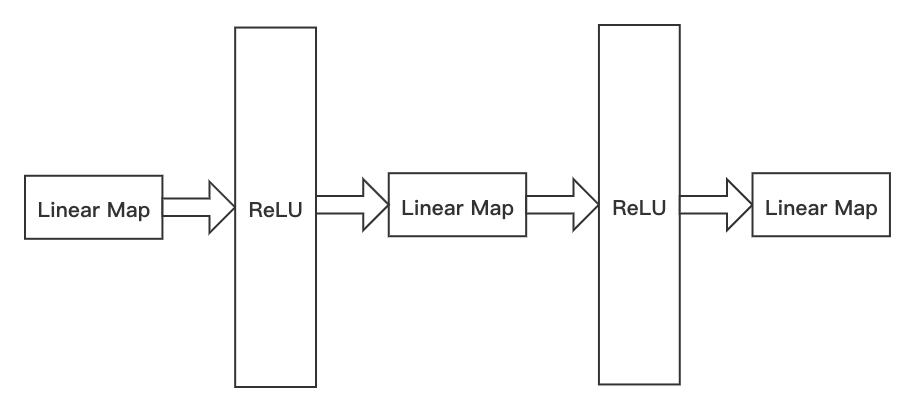
\includegraphics[scale=0.5]{images/onetask.png}


\subsection{Experiments (15 pts)}
In this section, we will train and test the two networks we implemented, and evaluate their performances.  

The network models will take images as inputs and give softmax output over 10 classes. During training, we will perform gradient descent with momentum to minimize Cross-Entropy Loss. Run the optimization for \textcolor{blue}{50} epochs each time. Using the following hyperparameters parameters for training: batch size = $128$, learning rate = $0.001$, momentum = $0.9$. %If you observe underfitting, continue training for more epochs until overfitting.

For every architecture, plot the train and test loss together on one plot, with loss on the y-axis against epoch number on x-axis. Similarly, plot the train and test accuracy after every epoch. Label each curve and all axes. Report the best loss and accuracy for training and testing achieved.

\pagebreak

\begin{enumerate}
    \item \textbf{(5 pts)} Train a \textbf{SingleLayerMLP} with $800$ hidden nodes, show plots of loss and accuracy, and report the best loss and accuracy achieved.
    \begin{soln}{height=9cm}
    \FiveBA
    \end{soln}

    \item \textbf{(5 pts)} Train a \textbf{TwoLayerMLP} with $(800, 800)$ hidden nodes, show plots of loss and accuracy, and report the best loss and accuracy achieved.
    \begin{soln}{height=9cm}
    \FiveBB
    \end{soln}
    \newpage
    
    \item \textbf{(3 pts)} Batch Normalization: To the \textbf{SingleLayerMLP} in Problem 1, implement batch normalization using the same batch size as in Problem 1. Describe how batch norm helps (or doesn't help) in terms of speed and accuracy (train and validation).
    \begin{soln}{height=9cm}
    \FiveBC
    \end{soln}

    \item \textbf{(2 pts)}  Dropout: Now, to the \textbf{SingleLayerMLP} of Problem 1, add a dropout to the output of layer 1 with a probability of 0.5 and report your findings. Do you observe any changes in terms of performance? Does a model trained with dropout perform better or worse than the SingleLayerMLP? Briefly explain why you think this happens.
    \begin{soln}{height=9cm}
    \FiveBD
    \end{soln}

\end{enumerate}